\chapter{Revisão de literatura}
\label{sec:revisao}
Este capítulo apresenta a fundamentação teórica para a compreensão de linha de produto de software (LPS) e gerenciamento de variabilidade com \textit{SMarty}, teste d LPS, teste baseado em modelo (TBM) e trabalhos relacionados com esta pesquisa.


\section{Linha de Produto de Software e a Abordagem SMarty}
\label{sec:conc_basicos}
O conceito de LPS tem como principal objetivo o desenvolvimento de sistemas que se baseiam em reutilização, e a migração para uma cultura de desenvolvimento onde novos sistemas são sempre derivados a partir de um conjunto de componentes e artefatos comuns, os quais constituem o núcleo da linha de produtos \cite{linden2007product}. 

Dessa maneira, além de componentes do núcleo, uma LPS inclui componentes responsáveis pela implementação de \textit{features} que são necessárias em determinados domínios ou ambientes de uso. Existem três modelos predominantes para criação de LPS: proativo, reativo e extrativo \cite{pohl2005software}.

O \textit{Software Engineering Institute} (SEI), por meio da iniciativa \textit{Product Line Practice} (PLP), define três atividades essenciais em LPS: o desenvolvimento do núcleo de artefatos, correspondente à engenharia de domínio; o desenvolvimento do produto, referente à engenharia de aplicação (\ref{fig:sei}.)

\begin{figure}[htb]
	\centering
	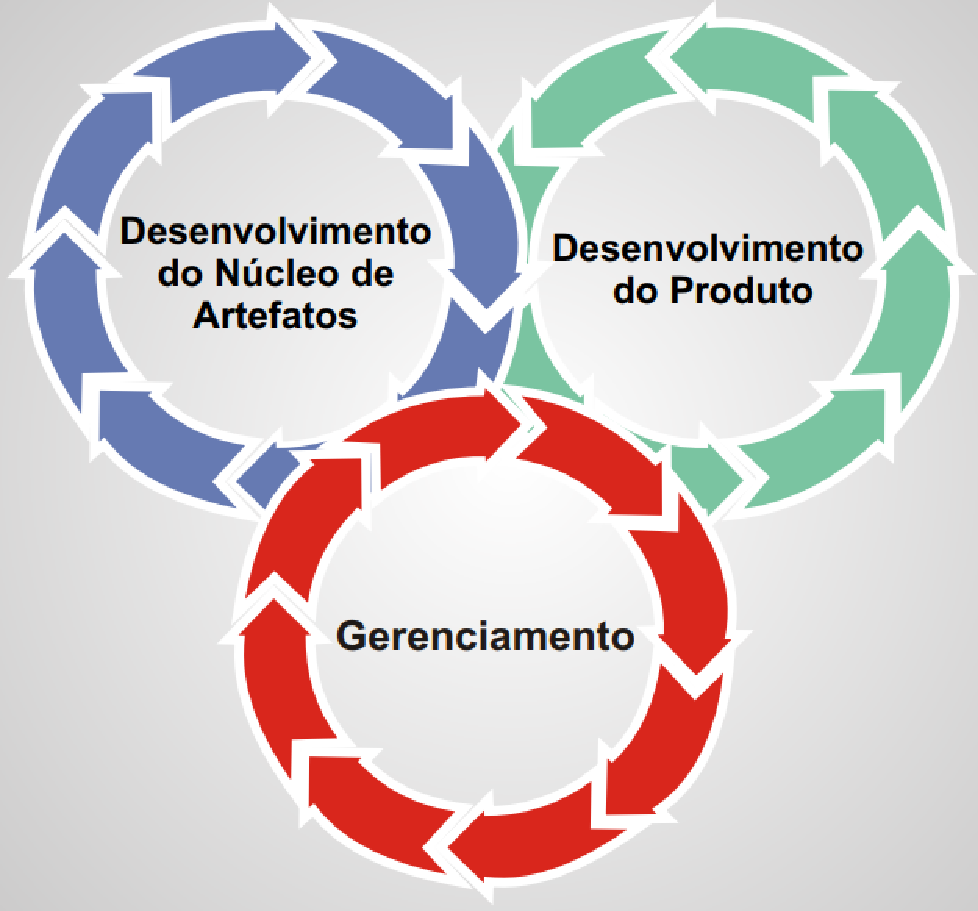
\includegraphics[scale=1.00]{sei.png}
	\caption{Adaptado de (SEI 2010) }
	\label{fig:sei}
\end{figure}
\newpage
\begin{itemize}
	\item \textbf{Engenharia de Domínio} processo em que as similaridades e as variabilidades das LPSs são identificadas e realizadas. No qual, é composto de cinco subprocessos principais, sendo eles: Gerenciamento de Produto, Engenharia de Requisitos do Domínio, Projeto do Domínio, Realização do Domínio e Teste de Domínio;
	\item \textbf{Engenharia de Aplicação} processo em que as aplicações de uma LPS são construídas por meio da reutilização de artefatos de domínio, explorando as variabilidades de uma linha de produto. No qual, é composto pelas subprocessos: Engenharia de Requisitos da Aplica¸c?ao, Projeto da Aplicação, Realização da Aplicação e Teste da Aplicação.
\end{itemize}

\cite{pohl2005software} desenvolveram um \textit{framework} para engenharia de LPS, cujo objetivo é incorporar os conceitos centrais da engenharia de linha de produto tradicional, proporcionando a reutilização de artefatos e a customização em massa por meio de variabilidades (\ref{fig:lps}).

\begin{figure}[htb]
	\centering
	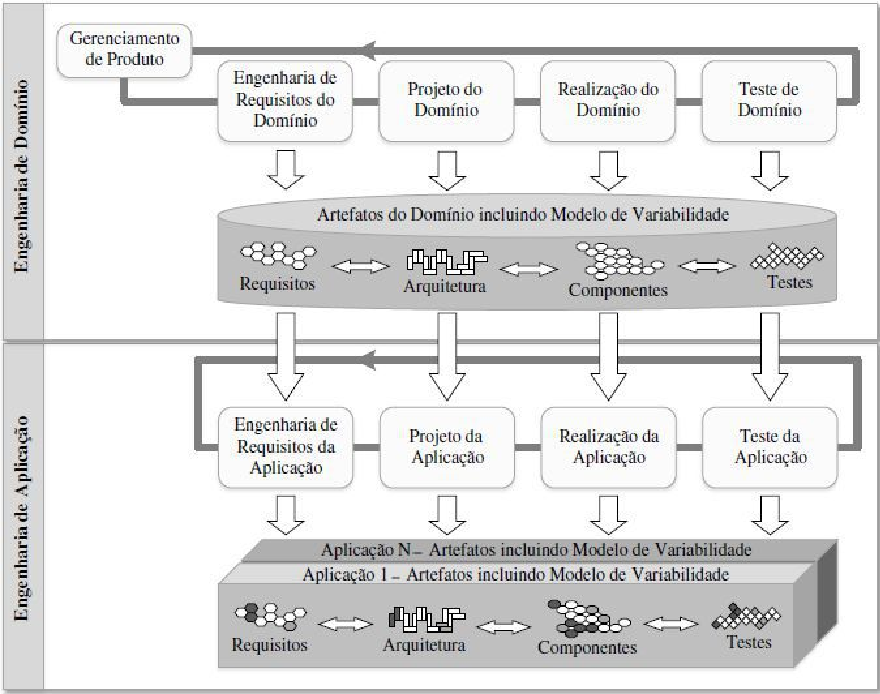
\includegraphics[scale=0.50]{lps.png}
	\caption{\textit{Framework} de Engenharia de LPS \cite{pohl2005software}. Traduzido por Geraldi (2015)}
	\label{fig:lps}
\end{figure}
\newpage
A adoção de LPS traz benefícios em diversos aspectos do processo de desenvolvimento de software, tais como \cite{linden2007product, pohl2005software}:

\begin{itemize}
	\item redução dos custos de desenvolvimento, devido ao re´uso de artefatos de um núcleo;
	\item melhoria da qualidade dos produtos, pois os artefatos produzidos são revisados e testados em vários produtos;
	\item redução do tempo de produção (\textit{time to market}) que é mais alto inicialmente, pois os artefatos comuns devem ser construídos antes. Mas, reduz ao produzir cada novo produto;
	\item redução do esforço de manutenção, pois quando um artefato do núcleo for modificado, as mudanças podem ser propagadas para todos os produtos que utilizam tal artefato;
	\item  contribuição para evolução, pois ao inserir um novo produto no núcleo da LPS, concede a oportunidade de evolução de todos os tipos de produtos derivados da LPS
	\item  contribuição para redução da complexidade, devido ao crescente número de solicitações de clientes, a complexidade dos produtos aumenta. Dessa forma, mais funcionalidades são adicionadas ao software. O fato de partes comuns serem
	reusadas por uma LPS ocorre a redução significativa da complexidade;
	\item melhoria na estimativa de custo, pois a organização pode se concentrar em promover produtos que são fáceis de ser gerados a partir da LPS e produtos que exijam extensões podem ser vendidos por preços mais altos; e 
	\item benefícios para os clientes, pois adquirem produtos adaptados às suas necessidades e expectativas por preços acessíveis devido a abordagem de LPS contribuir na redução
	de custos de desenvolvimento.
\end{itemize}

O núcleo de artefatos é composto de um conjunto de características comuns (similaridades) e características variáveis (variabilidades) \cite{linden2007product}. Esse núcleo forma a base da LPS e inclui a arquitetura de LPS, componentes reusáveis, modelos de domínios, requisitos da LPS, planos de testes e modelos de características e de variabilidades.

De acordo com Apel et al., (2013), "uma característica  é um
comportamento visível ao usuário final de um sistema de software". Uma característica pode ser obrigatória, opcional ou alternativa. O modelo de características representa as variabilidades de uma LPS Apel et al., (2013). Variabilidades são descritas por: Ponto de variação, o que permite a resolução de variabilidades em artefatos genéricos de uma LPS; Variante, que representa os possíveis elementos que podem ser escolhidos para resolver um ponto de variação e; Restrições entre variantes que estabelecem os relacionamentos entre uma ou mais variantes com o objetivo de resolver seus respectivos pontos de variação ou variabilidade em um dado tempo de resolução \cite{linden2007product,pohl2005software,apel2016feature}.

Analisando o contexto apresentado, podemos considerar que a variabilidade é algo muito importante para não ser levado em consideração quando falamos em qualidade de software. Existem várias abordagens para o gerenciamento de variabilidade, uma delas é a \textit{Stereotype-based Management of Variability} (\textit{SMarty}), que realiza o gerenciamento de variabilidades de uma LPS de forma clara e explícita em modelos UML \cite{junior2010systematic}. \textit{SMarty} é composta de um perfil UML, o \textit{SMartyProfile}, e do processo denominado \textit{SMartyProcess}. Ela guia o usuário por meio do \textit{SMartyProcess} na identificação e representação de variabilidades em modelos UML de uma LPS. O perfil \textit{SMartyProfile} é formado por um conjunto de estereótipos e meta-atributos para representar variabilidades em modelos UML de LPS.

Por meio da UML e seu mecanismo de perfil \textit{SMarty} permite a representação explícita de variabilidades. O \textit{SMartyProcess} é um processo sistemático que guia o usuário na identificação, delimitação, representação, rastreamento de variabilidades e análise de configurações de produtos de uma LPS (\ref{fig:smartyprocess}). Nele há um conjunto de diretrizes que permitem ao usuário a aplicação dos estereótipos do \textit{SMartyProfile} de forma clara e objetiva e é possível perceber todos os estereótipos suportados pelo perfil na região inferior da (\ref{fig:smartyprofile}). Mais informações relacionadas a \textit{SMarty} podem ser encontradas no anexo \ref{Abordagem_SMarty} - Abordagem \textit{SMarty}, assim como um exemplo de modelagem utilizando a abordagem.

\begin{figure}[htb]
	\centering
	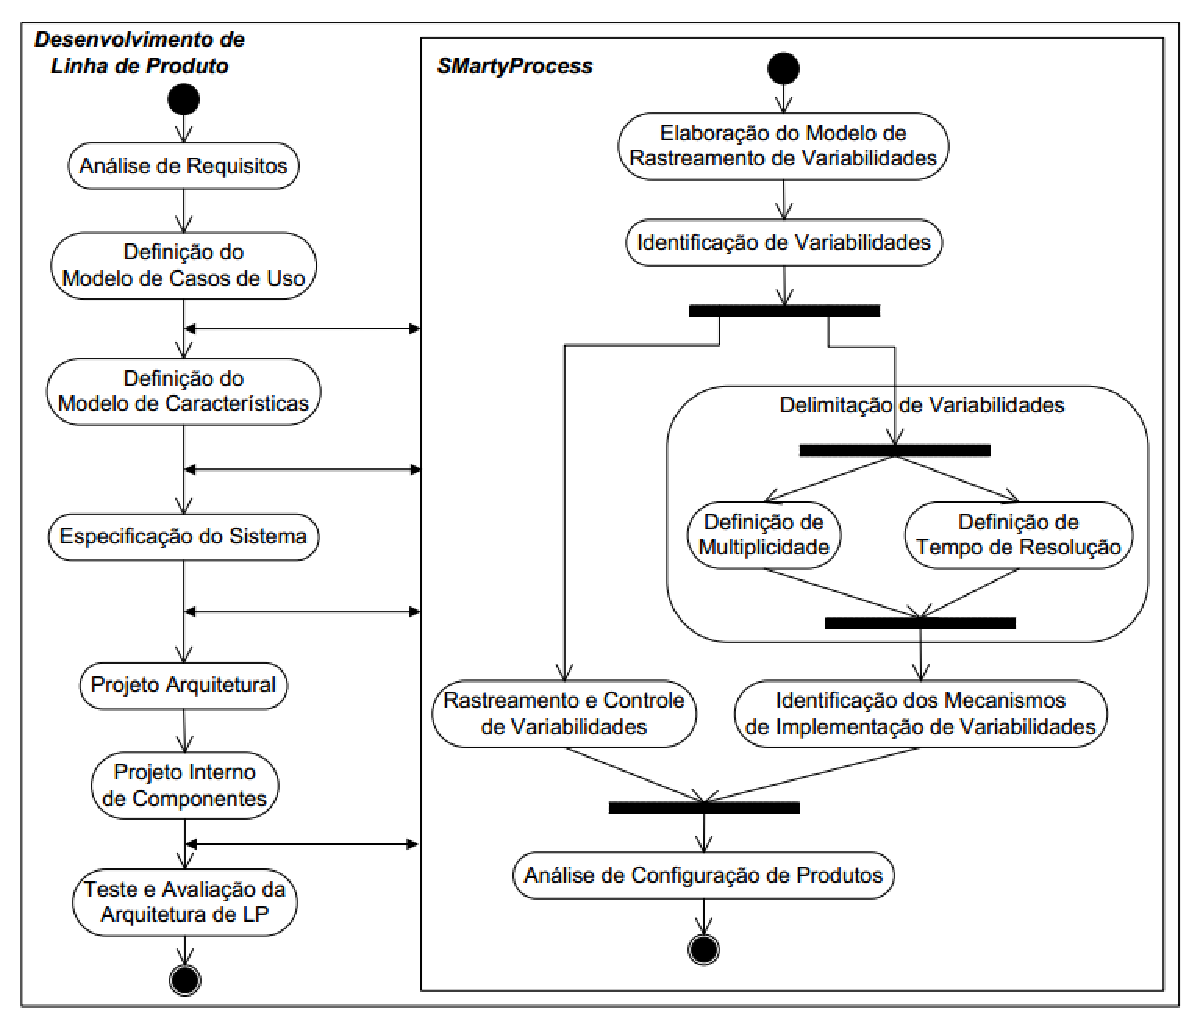
\includegraphics[scale=0.70]{smartyprocess.png}
	\caption{ O Processo de Gerenciamento de Variabilidades SMartyProcess e sua
		Interação entre as Atividades com o Processo de Desenvolvimento de LPS,
		traduzido de (OliveiraJr et al., 2010b)}
	\label{fig:smartyprocess}
\end{figure}

\newpage
\begin{landscape}

\begin{figure}[htb]
	\centering
	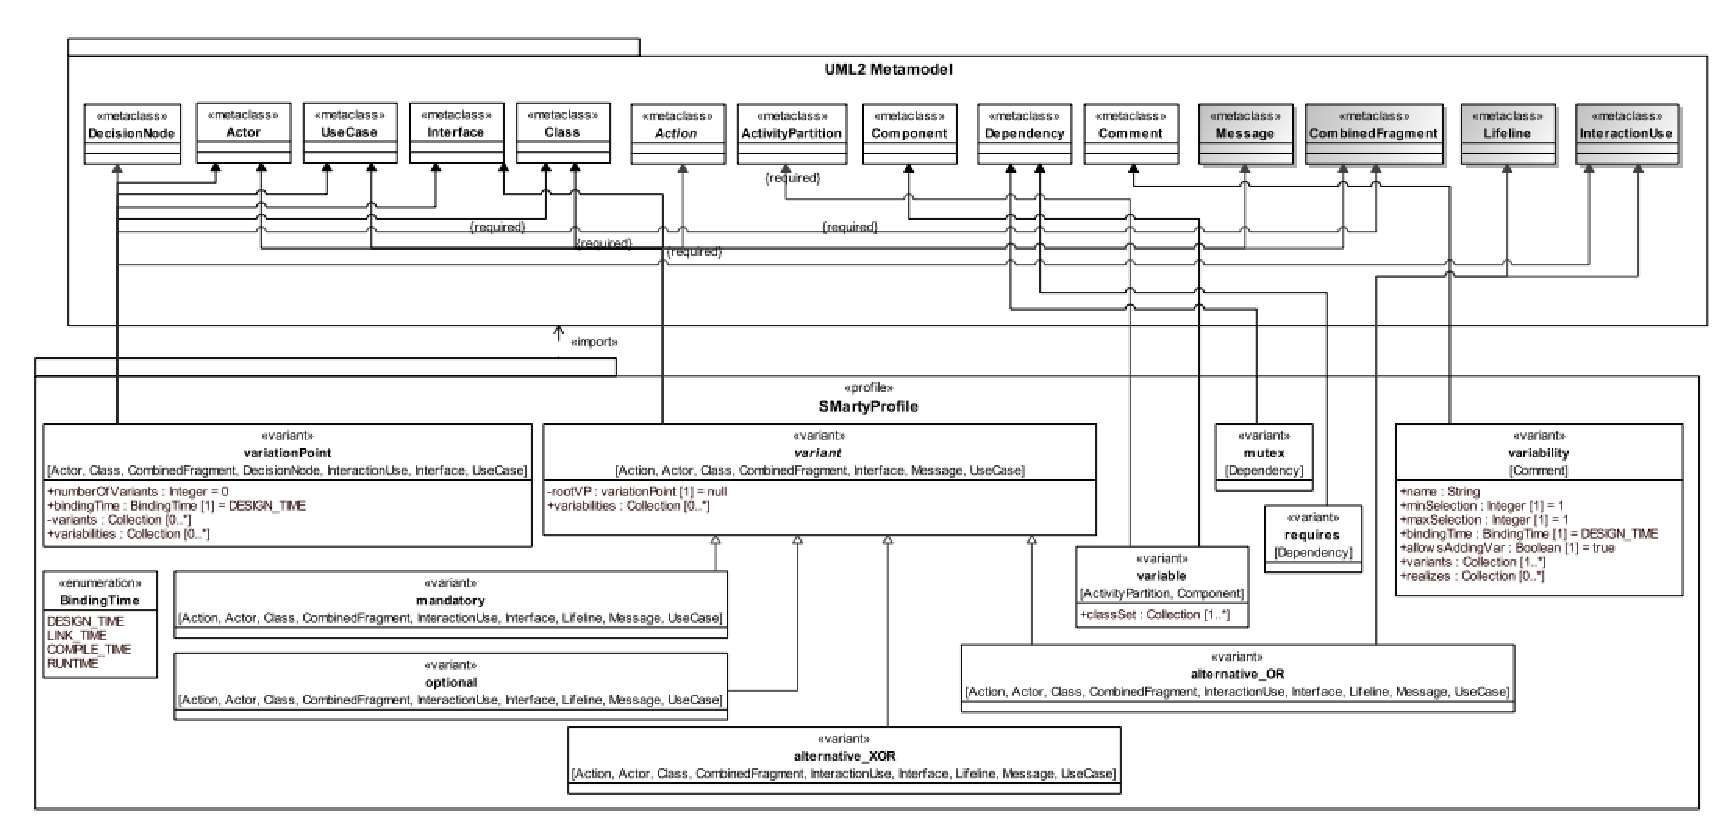
\includegraphics[scale=0.80]{smartyprofile.png}
	\caption{ Estereótipos e Meta-Atributos do Perfil SMartyProfile 5.1 com Suporte a Modelos de Casos de Uso, Classes, Componentes, Atividades e Sequência (Fiori et al., 2012; Marcolino, 2014; OliveiraJr et al., 2010a, 2013a). }
	\label{fig:smartyprofile}
\end{figure}


\end{landscape}

\section{Teste de Linha de Produto de Software e Teste Baseado em Modelo}
\label{sec:conc}
LPS é um interesse da indústria, pelo o potencial de reuso de artefatos além de aumentar a produtividade. Para alcançar as melhorias prometidas, a qualidade dos artefatos reutilizáveis deve ser verificado. Portanto, a garantia de qualidade em geral e os testes em particular, que ainda é a técnica de garantia de qualidade mais comum na indústria, são cruciais para os esforços de LPS \cite{delamaro2017introduccao}.

Sendo assim, para uma busca completa do desenvolvimento de teste em LPS primeiro temos que entender um processo de teste, existem vários modelos mas aqui iremos da um exemplo utilizando o modelo em V \ref{fig:teste}.

\begin{figure}[htb]
	\centering
	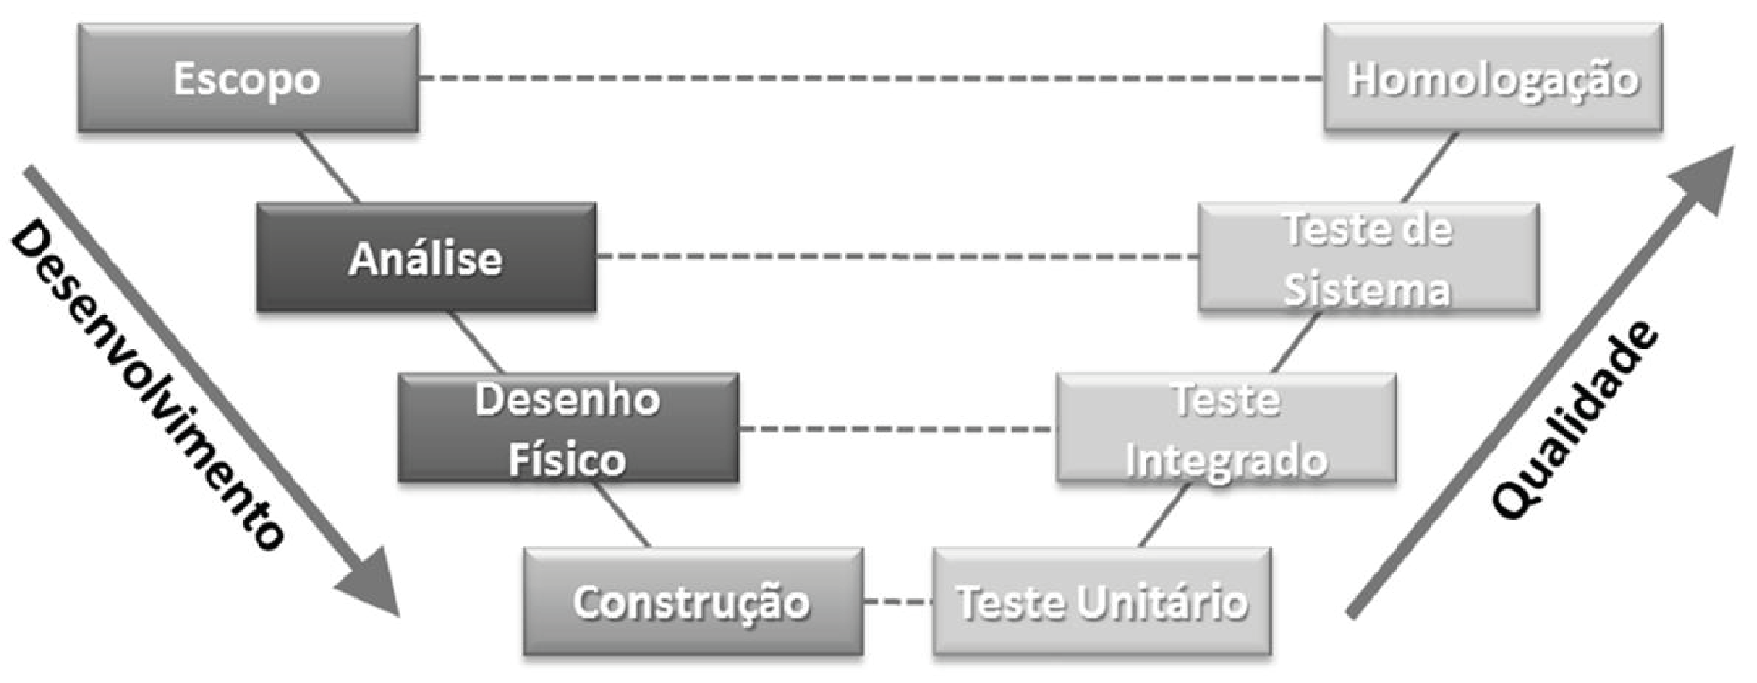
\includegraphics[scale=0.80]{teste.jpg}
	\caption{ Esquema simplificado que representa o modelo V }
	\label{fig:teste}
\end{figure}

Utilizando o modelo de teste consideramos duas etapas, a verificação e a validação. Em nosso trabalho iremos tratar a validação, e por se tratar de teste de funcionalidade em engenharia de domínio, iremos utilizar a técnica de caixa preta, onde sabe-se apenas o que entra e o esperado em sua saída, além do teste de funcionalidade.

\begin{figure}[htb]
	\centering
	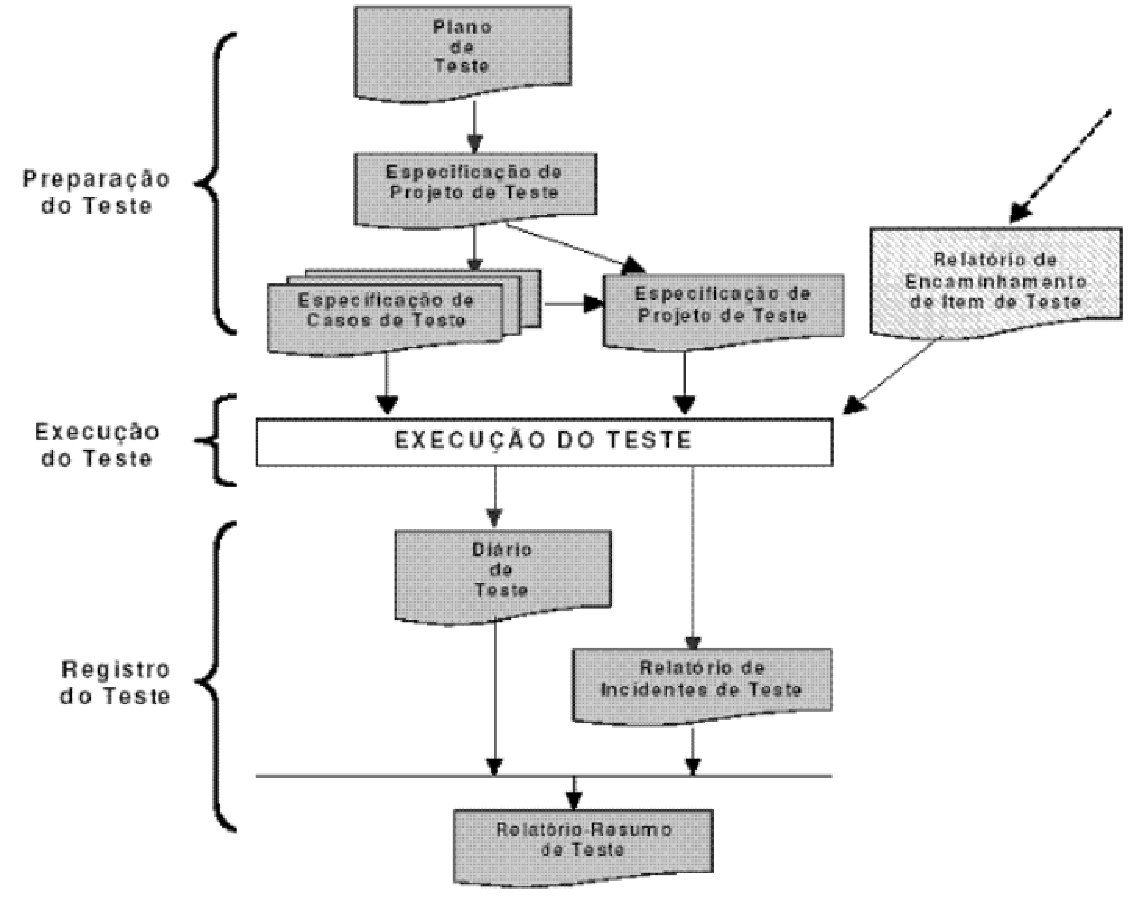
\includegraphics[scale=0.60]{testelps.png}
	\caption{ Modelo de proposta de implantação do processo de teste de software segundo \cite{crespo2004metodologia}}
	\label{fig:testelps}
\end{figure}

Sabendo-se que será utilizando teste caixa-preta o nível de teste abordado será o de sistema, restrito a funcionalidade do mesmo. Pensando neste sentido de trabalho de teste a nível de engenharia de Domínio procuramos buscar alternativas de teste que não necessitassem de atuação a nível de código ou caixa-branca.
\newpage
\citealp{do2014strategies} cita em um trabalho de revisão de literatura relacionando teste em LPS, buscam analisar as estratégias de testes que são abordadas e quais seus potenciais em uma maior taxa de detecção de erros. Nesse casso eles apontam que testes devem ser considerados tanto na engenharia de domínio como na de aplicação e dentro do interesse de teste dois itens devem ser levados em consideração, o conjunto de requisitos do produto e a qualidade do modelo de variabilidade em teste.

\cite{do2014strategies} apresentam um grande número de técnicas para lidar com o aspecto de seleção de produto para teste e o teste real dos produtos. No entanto, faltam relatos reais de experiências industriais que limitam algumas conclusões. O estudo ainda apresenta uma série de estratégias que podem apoiar a seleção e a execução dos testes reais em produtos.

O Teste Baseado em Modelo (TBM) é uma forma de teste de software em que os casos de teste são derivados de um modelo que descreve aspectos (geralmente funcionais) do sistema sendo testado. Tais casos são conhecidos como a suíte abstrata de testes, e seu nível de abstração está intimamente relacionado ao nível de abstração do modelo \cite{do2014strategies}. As vantagens da abordagem é que a geração de testes começa mais cedo no ciclo do desenvolvimento e pode-se criar casos de teste automaticamente a partir do modelo. 

Os casos de teste podem ser representados por meio de árvores de decisão, \textit{statecharts}, ontologias de domínio ou diagramas de casos de uso e/ou estados da UML (\textit{Unified Modeling Language})\cite{isa2017model}.

Um dos maiores desafios em teste de LPS se dá em relação as particularidades de cada modelo, para isso TBM busca na criação de modelos dentro da engenharia de domínio, realizar a geração de casos de teste que possam ser reutilizados na engenharia de aplicação. Alguns trabalhos realizados focam na construção da geração antecipada dos teste na modelagem de domínio da LPS, onde, o foco das pesquisas ficam em relação a como conseguir gerar reutilização com uma maior cobertura dos possíveis problemas.

TBM se faz de uso de Máquinas de Estado Finito (MEF), um modelo formal que representa as possíveis configurações do sistema.

\begin{figure}[htb]
	\centering
	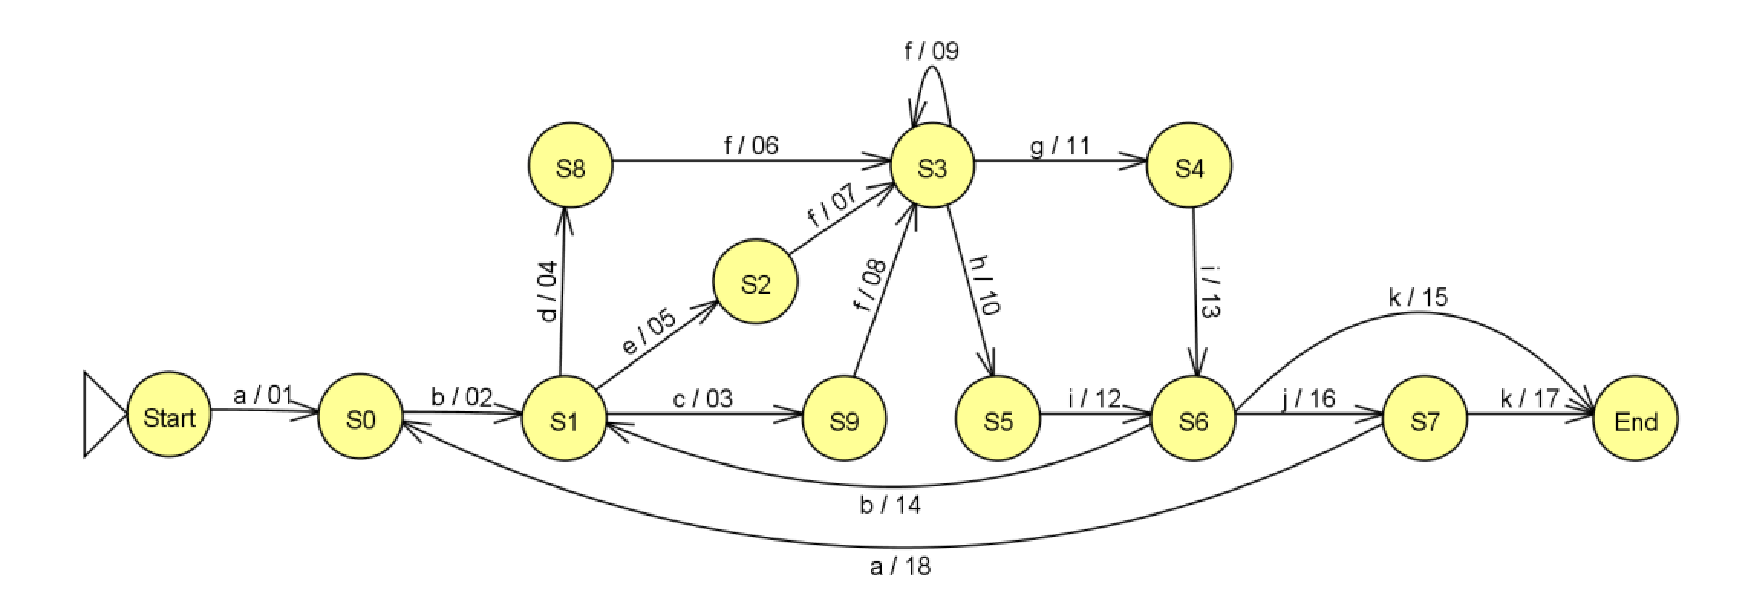
\includegraphics[scale=0.50]{fsm.png}
	\caption{ Exemplo de uma FSM \citealp{costa2016split}}
	\label{fig:testetbm}
\end{figure}


Sabendo que TBM possui características favoráveis na utilização em LPS e que proporciona uma certa relação com variabilidade, foi conduzido uma RSL com este propósito. Onde, ao longo de toda a RSL (Apêndice A) foram encontrados vários estudos que indicam a utilizam de TBM para LPS com tratativa da variabilidade.

Os estudos reportam que a partir de um modelo é realizado a conversão para um artefato, normalmente máquina de estado finito, assim, ele pode ser verificado os pontos de variação e variabilidade. Após, gerenciado essa variabilidade com ou sem a utilização de uma ferramenta de apoio. E por fim, a criação do caso de teste, fazendo o uso ou não de rastreabilidade.

Para facilitar a leitura os estudos utilizados para a extração de dados estão contidos na \ref{table:listaextraquali} e um guia visual na \ref{fig:guiaestudoquali}. Porém, caso o leitor queira mais detalhes sobre o guia ou os trabalhos, ele pode consultar a RSL no (Apêndice A)


\begin{landscape}
	\scalefont{0.7}
	\begin{longtable}[c]{|c|l|l|c|c|c|}
		\caption{Trabalhos selecionados para leitura e extração de dados}
		\label{table:listaextraquali}\\
		\hline
		\textbf{ID} & \multicolumn{1}{c|}{\textbf{Título}} & \multicolumn{1}{c|}{\textbf{Autor(res)}} & \textbf{\begin{tabular}[c]{@{}c@{}}Ano de \\ Publicação\end{tabular}} & \textbf{Fonte} & \textbf{Tipo} \\ \hline
		\endfirsthead
		%
		\hline
		\textbf{ID} & \multicolumn{1}{c|}{\textbf{Título}} & \multicolumn{1}{c|}{\textbf{Autor(res)}} & \textbf{\begin{tabular}[c]{@{}c@{}}Ano de \\ Publicação\end{tabular}} & \textbf{Fonte} & \textbf{Tipo} \\ \hline
		
		\endhead
		%
		T1 & \begin{tabular}[c]{@{}l@{}}Delta-Oriented Model-Based \\ SPL Regression Testing\end{tabular} & \begin{tabular}[c]{@{}l@{}}Sascha Lity, Malte Lochau, \\ Ina Schaefer, Ursula Goltz\end{tabular} & 2012 & ACM & Evento \\ \hline
		T2 & \begin{tabular}[c]{@{}l@{}}Industrial Evaluation of Pairwise \\ SPL Testing with MoSo-PoLiTe\end{tabular} & \begin{tabular}[c]{@{}l@{}}Michaela Steffens, Sebastian Oster, \\ Malte Lochau, Thomas Fogdal\end{tabular} & 2012 & ACM & Evento \\ \hline
		T3 & \begin{tabular}[c]{@{}l@{}}Model-Based Coverage-Driven Test Suíte \\ Generation for Software Product Lines\end{tabular} & \begin{tabular}[c]{@{}l@{}}Harald Cichos, Sebastian Oster, \\ Malte Lochau, Andy Schurr\end{tabular} & 2011 & ACM & Periódico \\ \hline
		T4 & \begin{tabular}[c]{@{}l@{}}MoSo-PoLiTe - Tool Support for \\ Pairwise and Model-Based Software \\ Product Line Testing\end{tabular} & \begin{tabular}[c]{@{}l@{}}Sebastian Oster, Ivan Zorcic, \\ Florian Markert, Malte Lochau\end{tabular} & 2011 & ACM & Evento \\ \hline
		T5 & MPLM - MaTeLo Product Line Manager & Hamza Samih, Ralf Bogusch & 2014 & ACM & Evento \\ \hline
		T6 & \begin{tabular}[c]{@{}l@{}}On the use of test cases in model-based \\ software product line development\end{tabular} & \begin{tabular}[c]{@{}l@{}}Alexander Knapp, Markus Roggenbach, \\ Bernd-Holger Schlingloff\end{tabular} & 2014 & ACM & Evento \\ \hline
		T7 & \begin{tabular}[c]{@{}l@{}}Pairwise Feature-Interaction Testing \\ for SPLs: Potentials and Limitations\end{tabular} & \begin{tabular}[c]{@{}l@{}}Sebastian Oster, Malte Lochau, \\ Marius Zink, Mark Grechanik\end{tabular} & 2011 & ACM & Evento \\ \hline
		T8 & \begin{tabular}[c]{@{}l@{}}Deriving Usage Model Variants for \\ Model- based Testing: An Industrial Case Study\end{tabular} & \begin{tabular}[c]{@{}l@{}}Hamza Samih,  Hélène Le Guen, \\ Ralf Bogusch, Mathieu Acher, Benoit Baudry\end{tabular} & 2014 & IEEE & Evento \\ \hline
		T9 & \begin{tabular}[c]{@{}l@{}}Model-based Software Product Line \\ Testing by Coupling Feature Models \\ with Hierarchical Markov Chain Usage Models\end{tabular} & Ceren Sahin Gebizli, Hasan Sozer & 2016 & IEEE & Evento \\ \hline
		T10 & \begin{tabular}[c]{@{}l@{}}Model-Based Test Design of Product Lines: \\ Raising Test Design to the Product Line Level\end{tabular} & \begin{tabular}[c]{@{}l@{}}Hartmut Lackner, Martin Thomas, \\ Florian Wartenberg, Stephan Weißleder\end{tabular} & 2014 & IEEE & Periódico \\ \hline
		T11 & Requirements-Based Delta-Oriented SPL Testing & \begin{tabular}[c]{@{}l@{}}Michael Dukaczewski, Ina Schaefer, \\ Remo Lachmann, Malte Lochau\end{tabular} & 2013 & IEEE & Evento \\ \hline
		T12 & \begin{tabular}[c]{@{}l@{}}Using Feature Model to Support Model- Based \\ Testing of Product Lines: An Industrial Case Study\end{tabular} & \begin{tabular}[c]{@{}l@{}}Shuai Wang,  Shaukat Ali,\\  Tao Yue, Marius Liaaen\end{tabular} & 2013 & IEEE & Periódico \\ \hline
		T13 & \begin{tabular}[c]{@{}l@{}}An automated Model-based Testing \\ Approach in Software Product Lines \\ Using a Variability Language\end{tabular} & \begin{tabular}[c]{@{}l@{}}Boni García,  Rodrigo García-Carmona, \\ Álvaro Navas, Hugo A. Parada-Gélvez,\\  Félix Cuadrado, Juan C. Dueñas\end{tabular} & 2010 & \begin{tabular}[c]{@{}c@{}}Politécnica \\ Arquivo \\ digital UPM\end{tabular} & Evento \\ \hline
		T14 & \begin{tabular}[c]{@{}l@{}}Automated Product Line Methodologies \\ to Support Model-Based Testing\end{tabular} & Shuai Wang,  Shaukat Ali, Arnaud Gotlieb & 2013 & \begin{tabular}[c]{@{}c@{}}CEUR \\ Event Proceedings\end{tabular} & Evento \\ \hline
		T15 & \begin{tabular}[c]{@{}l@{}}Behavioural Model Based \\ Testing of Software Product Lines\end{tabular} & Xavier Devroey & 2014 & ACM & Evento \\ \hline
		T16 & \begin{tabular}[c]{@{}l@{}}Feature Model-based \\ Software Product Line Testing\end{tabular} & SEBASTIAN OSTER & 2012 & TUprints & Periódico \\ \hline
		T17 & \begin{tabular}[c]{@{}l@{}}Model-based pairwise testing for feature interaction \\ coverage in software product line engineering\end{tabular} & \begin{tabular}[c]{@{}l@{}}Malte Lochau, Sebastian Oster, \\ Ursula Goltz, Andy Schurr\end{tabular} & 2011 & Springer & Periódico \\ \hline
		T18 & Model-based Test Generation for Software Product Line & Xinying Cai, Hongwei Zeng & 2013 & IEEE & Evento \\ \hline
		T19 & Model-Based Testing for Software Product Lines & Erika Mir Olimpiew & 2008 & Springer & Evento \\ \hline
		T20 & PLETS - A Product line of model-based testing tools & Elder de Macedo Rodrigues & 2013 & PUC-RS & Evento \\ \hline
		T21 & \begin{tabular}[c]{@{}l@{}}Top-Down and Bottom-Up Approach for \\ Model-Based Testing of Product Lines\end{tabular} & Stephan Weißleder, Hartmut Lackner & 2013 & EPTCS & Evento \\ \hline
		T22 & \begin{tabular}[c]{@{}l@{}}A Product Line Modeling and Configuration  Methodology \\ to Support Model-Based  Testing: An Industrial Case Study\end{tabular} & \begin{tabular}[c]{@{}l@{}}Shaukat Ali, Tao Yue, Lionel Briand, \\ Suneth Walawege\end{tabular} & 2012 & Springer & Periódico \\ \hline
		T23 & \begin{tabular}[c]{@{}l@{}}Coverage Criteria for Behavioural \\ Testing of Software Product Lines\end{tabular} & \begin{tabular}[c]{@{}l@{}}Xavier Devroey, Gilles Perrouin, \\ Axel Legay, Maxime Cordy, \\ Pierre-Yves Schobbens, Patrick Heymans\end{tabular} & 2014 & Springer & Evento \\ \hline
		T24 & \begin{tabular}[c]{@{}l@{}}A Model Based Testing Approach for Model-Driven \\ Development and Software Product Lines\end{tabular} & \begin{tabular}[c]{@{}l@{}}Beatriz Pérez Lamancha,  Macario Polo Usaola, \\ Mario Piattini Velthius\end{tabular} & 2010 & Springer & Evento \\ \hline
		T25 & \begin{tabular}[c]{@{}l@{}}A Vision for Behavioural Model-Driven \\ Validation of Software Product Lines\end{tabular} & \begin{tabular}[c]{@{}l@{}}Xavier Devroey, Maxime Cordy,  \\ Gilles Perrouin, Eun-Young Kang, \\ Pierre-Yves Schobbens, Patrick Heymans, \\ Axel Legay,  Benoit Baudry\end{tabular} & 2012 & Springer & Evento \\ \hline
		T26 & \begin{tabular}[c]{@{}l@{}}Abstract Test Case Generation for Behavioural \\ Testing of Software Product Lines\end{tabular} & \begin{tabular}[c]{@{}l@{}}Xavier Devroey, Gilles Perrouin, \\ Pierre-Yves Schobbens\end{tabular} & 2014 & ACM & Evento \\ \hline
		T27 & \begin{tabular}[c]{@{}l@{}}Applying Incremental Model Slicing to \\ Product-Line Regression Testing\end{tabular} & \begin{tabular}[c]{@{}l@{}}Sascha Lity, Thomas Morbach,  \\ Thomas Th¨ um, Ina Schaefer\end{tabular} & 2016 & Springer & Periódico \\ \hline
		T28 & \begin{tabular}[c]{@{}l@{}}Automated Testing of Software-as- a-Service \\ Configurations using a Variability Language\end{tabular} & Sachin Patel, Vipul Shah & 2015 & ACM & Evento \\ \hline
		T29 & Delta-Oriented FSM-Based Testing & \begin{tabular}[c]{@{}l@{}}Mahsa Varshosaz,  Harsh Beohar, \\ Mohammad Reza Mousavi\end{tabular} & 2015 & Springer & Evento \\ \hline
		T30 & \begin{tabular}[c]{@{}l@{}}Incremental Model-Based Testing of \\ Delta-oriented Software Product Lines\end{tabular} & \begin{tabular}[c]{@{}l@{}}Malte Lochau, Ina Schaefer, \\ Jochen Kamischke, Sascha Lity\end{tabular} & 2012 & Springer & Periódico \\ \hline
		T31 & Model Based Testing in Software Product Lines & \begin{tabular}[c]{@{}l@{}}Pedro Reales, Macario Polo, \\ Danilo Caivano\end{tabular} & 2011 & Springer & Evento \\ \hline
		T32 & Model-Based Testing & \begin{tabular}[c]{@{}l@{}}Malte Lochau, Sven Peldszus, \\ Matthias Kowal,  Ina Schaefer\end{tabular} & 2014 & Springer & Evento \\ \hline
		T33 & \begin{tabular}[c]{@{}l@{}}Parameterized Preorder Relations for \\ Model-Based Testing of Software Product Lines\end{tabular} & Malte Lochau, Jochen Kamischke & 2012 & Springer & Evento \\ \hline
		T34 & Poster: VIBeS, Transition System Mutation Made Easy & \begin{tabular}[c]{@{}l@{}}Xavier Devroey, Gilles Perrouin, \\ Pierre-Yves Schobbens, Patrick Heymans\end{tabular} & 2015 & IEEE & Evento \\ \hline
		T35 & Spinal Test Suites for Software Product Lines & Harsh Beohar, Mohammad Reza Mousavi & 2014 & EPTCS & Evento \\ \hline
		T36 & \begin{tabular}[c]{@{}l@{}}Automated model-based testing\\ using the  UML testing profile and QVT\end{tabular} & \begin{tabular}[c]{@{}l@{}}Beatriz Pérez Lamancha, Pedro Reales Mateo, \\ IgnacioRodríguez de Guzmán, Macario Polo Usaola, \\ Mario Piattini Velthius\end{tabular} & 2009 & ACM & Evento \\ \hline
		T37 & \begin{tabular}[c]{@{}l@{}}Relating Variability Modeling and \\ Model- Based Testing for Software Product Lines Testing\end{tabular} & Hamza Samih & 2012 & ICTSS & Evento \\ \hline
		T38 & \begin{tabular}[c]{@{}l@{}}An Evaluation of Model-Based \\ Testing in Embedded Applications\end{tabular} & Stephan Weißleder, Holger Schlingloff & 2014 & IEEE & Evento \\ \hline
		T39 & \begin{tabular}[c]{@{}l@{}}Assessing Software Product Line Testing Via Model-Based \\ Mutation An Application to Similarity Testing\end{tabular} & \begin{tabular}[c]{@{}l@{}}Christopher Henard, Mike Papadakis, \\ Gilles Perrouin, Jacques Klein, Yves Le Traon\end{tabular} & 2013 & IEEE & Evento \\ \hline
		T40 & \begin{tabular}[c]{@{}l@{}}Automated and Scalable T-wise Test Case Generation \\ Strategies for Software Product Lines\end{tabular} & \begin{tabular}[c]{@{}l@{}}Gilles Perrouin, Sagar Sen, Jacques Klein, \\ Benoit Baudry, Yves le Traon Lassy\end{tabular} & 2010 & IEEE & Evento \\ \hline
		T41 & \begin{tabular}[c]{@{}l@{}}Model-based Testing of System Requirements \\ using UML Use Case Models\end{tabular} & Bill Hasling, Helmut Goetz, Klaus Beetz & 2008 & IEEE & Evento \\ \hline
		T42 & \begin{tabular}[c]{@{}l@{}}Successive refinement of models for model-based \\ testing to increase system test effectiveness\end{tabular} & \begin{tabular}[c]{@{}l@{}}Ceren Sahin Gebizli, Hasan Sozer, \\ Ali Ozer Ercan\end{tabular} & 2016 & IEEE & Evento \\ \hline
		T43 & A Software Product Line for Model-Based Testing Tools & \begin{tabular}[c]{@{}l@{}}Elder M. Rodrigues, Avelino F. Zorzo, \\ Itana M. Gimenez, Elisa Y. Nakagawa, \\ Flavio M. Oliveira, José C. Maldonado\end{tabular} & 2012 & PUC-RS & Outro \\ \hline
		T44 & \begin{tabular}[c]{@{}l@{}}Reusing State Machines for Automatic \\ Test Generation in Product Lines\end{tabular} & \begin{tabular}[c]{@{}l@{}}Stephan Weißleder, Dehla Sokenou, \\ Bernd-Holger Schlingloff\end{tabular} & 2008 & MoTip & Evento \\ \hline
	\end{longtable}
\end{landscape}



\begin{landscape}
	
	\begin{figure}[htb]
		\centering
		\caption{Guia de estágios do processo de TBM em LPS}
		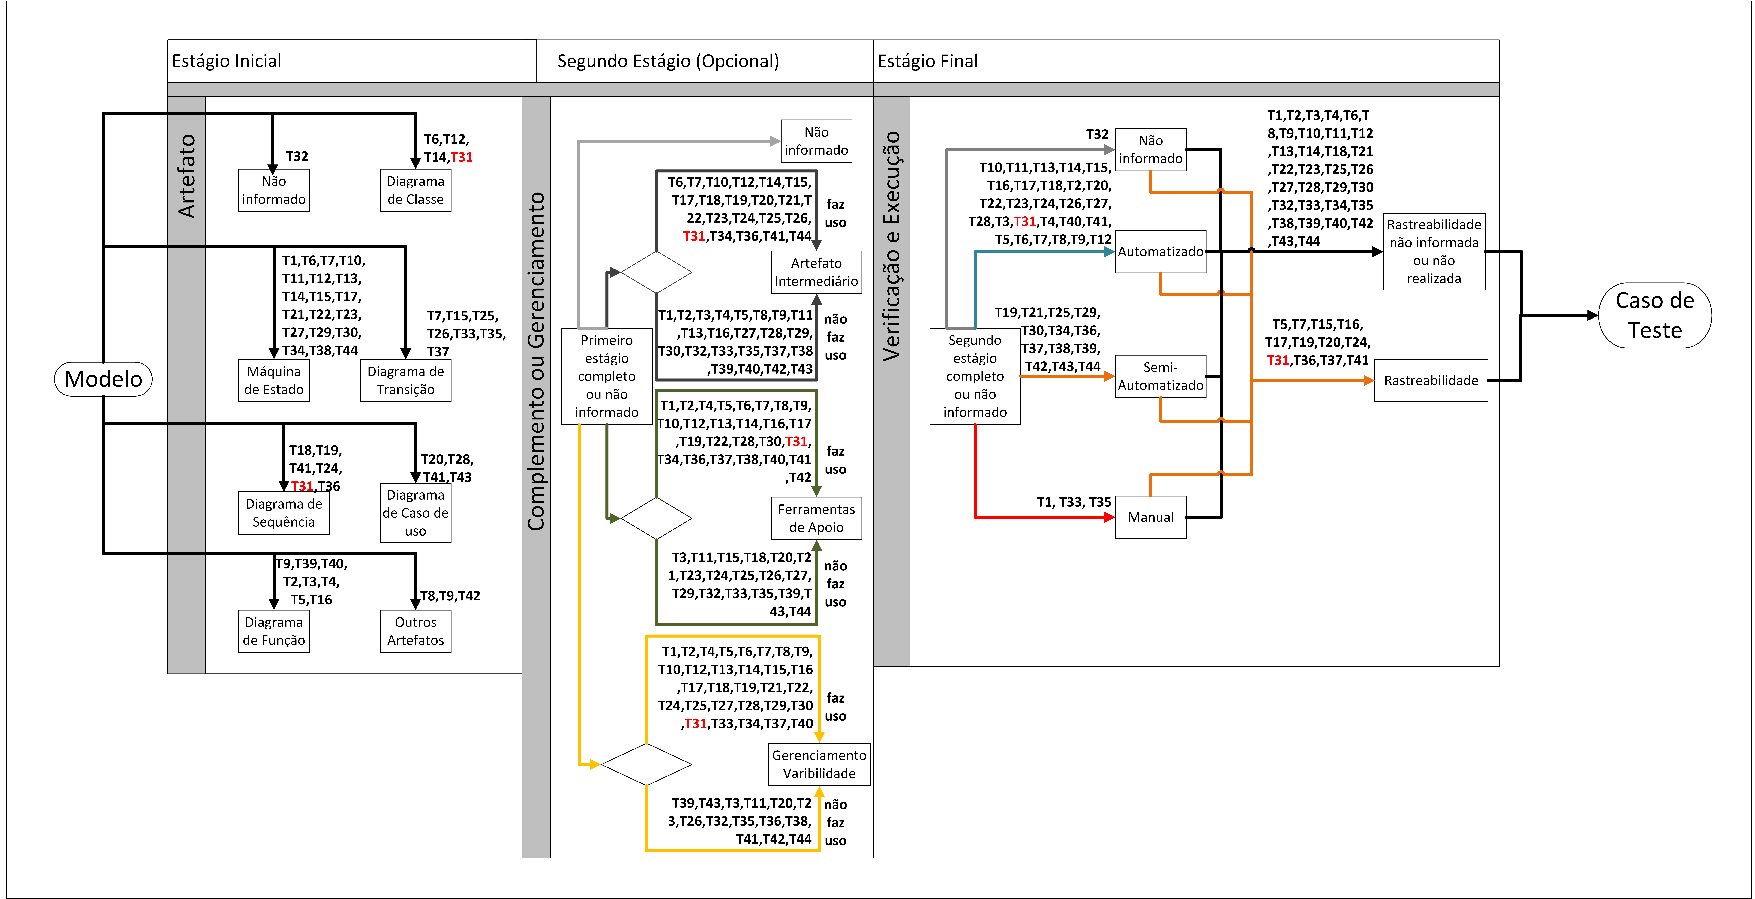
\includegraphics[scale=0.40]{guiaestudo.jpg}
		\label{fig:guiaestudoquali}
	\end{figure}
	
\end{landscape}


\section{Trabalhos relacionados}
\label{sec:conc_basi}
Utilizando a RSL conduzida obtivemos dados e indicadores que conduzissem esta pesquisa e em seguida apresentamos alguns trabalhos que se mostram referência para o embasamento cientifico experimental.

\cite{costa2016split} apresenta um método chamada SPLiT-MBt onde é possível gerar casos de teste funcional e \textit{scripts} para testar os produtos derivados de uma LPS, onde os casos de teste comuns entre os produtos derivados são gerados com base no reuso inerente a LPS.

Para fornecer o reuso ele é aplicado em duas etapas, onde a primeira é realizada a anotação em modelo de sistema as informações de variabilidade e teste, e em seguida utilizadas para gerar sequências de teste usando diferentes métodos. O modelo formal utilizado é Máquina de Estado Finito e que são estendidas para lidar com as informações sobre variabilidade.

Já na segunda etapa, os modelos de teste e as sequências geradas são utilizadas para gerar os \textit{scripts} de teste que podem ser executados por diferentes ferramentas de teste funcional. SPLiT-MBt faz uso da abordagem \textit{SMarty} para o gerenciamento de variabilidade, porém, a diferença desta abordagem para a \textit{SMartyTesting} é que ela dará suporte a dois modelos a mais, diagrama de caso de uso e de sequência.

(FRAGAL, V. H., 2017) busca automatizar a geração de pequenos conjuntos de teste com alta capacidade de detecção de falhas e baixa redundância de teste entre produtos. Para isso, testes equivalentes são identificados e reutilizados em um conjunto de produtos e utilizando conjuntos de testes configuráveis.

A pesquisa realizada foi dividida em duas direções, a primeira centrada no produto e a segunda na arquitetura reutilizável. Os conjuntos de teste citados anteriormente, são gerados para garantir cobertura completa de falhas, geradas a partir de máquinas de estado finito e, para o gerenciamenot de variabilidade eles utilizam no momento da modelagem o modelo de variabilidade ortogonal (OVM). Da mesma forma que o trabalho de (Costa, L. T., 2016), este faz somente uso de máquinas de estado finito, portanto, o que diferencia do nosso trabalho é a utilização de mais dois tipos de modelos formais ao apoio da abordagem \textit{SMarty}.

Seguindo a geração de casos de teste a partir da SPL, \cite{cai2013model} trazem uma abordagem baseada em modelo para testar geração de casos de testes para SPLs, onde possa ser reutilizável esses cenários de teste e de domínio que são gerados a partir de diagramas de atividades estendido com pontos de variação e, em seguida, teste dos cenários de acordo com os pontos de variação. Este trabalho contribui para identificarmos as situações de geração a partir de caso de teste, porém não deixa claro como é feito o tratamento de variabilidade.

\cite{olimpiew2008model} também proporciona muito dados e informações sobre o TBM em LPS, embora o foco seja em diagramas de atividades customizadas, mas com um foco na reutilização do teste em produtos variantes da LPS. A abordagem proposta CADeT, transforma os casos de uso em diagramas de atividades e que por sua vez são transformados em casos de teste. As especificações de teste são rastreadas a partir do diagrama de atividade e do caso de uso. A contribuição seria relacionada ao processo de reutilização de caso de teste conforme a mudança de característica do produto, pois segundo a abordagem, pode ser usado para criar especificações de teste reutilizáveis para cobrir todos cenários de casos de uso.

Já \cite{lamancha2010model} utiliza o modelo de variabilidade Ortogonal OVM, já os modelos são convertidos em modelos de design e a partir deles são gerados os modelos de teste. Diferente da proposta deste trabalho, o gerenciamento de variabilidade é realizado na modelagem apenas uma vez. \cite{reales2011model},\cite{lochau2012parameterized}, e \cite{samih2012relating} Trabalham diretamente dos modelos por diagrama de sequência e são exclusivamente utilizados para a geração dos diagramas necessários para a criação dos casos de teste, e no quesito de variabilidade é modelado utilizando notação ortogonal OVM. Já \cite{weissleder2014evaluation} trabalha a partir do modelo mas não faz uso de OVM, ambos utilizam OVM para o tratamento de variabilidade.

\cite{hasling2008model} realiza a conversão dos modelos em diagramas de atividade e caso de uso, após essa conversão é trabalhado a criação de casos de teste, onde as variantes dos modelos podem ser considerados como variáveis, mas não relata como e onde esse ponto é tratado durante o processo. De forma similar \cite{gebizli2016successive} trabalha o modelo refinando até se chegar aos processos de transições, mas não menciona se é tratada a variabilidade ou como seria tratado, o foco fica somente nos modelos.

Uma comparação entre os trabalhos mencionados anteriormente pode ser analisada na \ref{table:lista}

\begin{landscape}
	\begin{table}[]
		\caption{Relação de comparação dos trabalhos relacionados}
		\label{table:lista}
		\resizebox{1.6\textwidth}{!}{%
			\begin{tabular}{|l|l|l|l|l|l|l|l|l|l|l|}
				\hline
				\textbf{Título} & \textbf{Autor(res)} & \textbf{Ano} & \textbf{\begin{tabular}[c]{@{}l@{}}Considera \\ \\ Variabilidade?\end{tabular}} & \textbf{\begin{tabular}[c]{@{}l@{}}Nível\\ de Teste\end{tabular}} & \textbf{Técnica de Teste} & \textbf{\begin{tabular}[c]{@{}l@{}}Abordagem \\ \\ de Teste\end{tabular}} & \textbf{\begin{tabular}[c]{@{}l@{}}Faz uso de Artefato\\ Intermediário\end{tabular}} & \textbf{\begin{tabular}[c]{@{}l@{}}Utilização de \\ \\ ferramenta de apoio\end{tabular}} & \textbf{\begin{tabular}[c]{@{}l@{}}Local de \\ \\ Validação\end{tabular}} & \textbf{Tipo de Contribuição} \\ \hline
				\begin{tabular}[c]{@{}l@{}}SPLiT-MBT: A Model-Based Testing \\ Method for Software Product Lines\end{tabular} & Leandro Teodoro Costa & 2017 & Sim & Sistema & Caixa Preta & Semi automatizada & Máquina de Estado Finito & SPLiT-MBT & Acadêmia & Abordagem \\ \hline
				\begin{tabular}[c]{@{}l@{}}Automatic generation of configurable \\ test-suites for software product lines\end{tabular} & Vanderson Hafemann Fragal & 2017 & Sim & Sistema & Caixa Preta & Automatizada & Máquina de Estado Finito & Não mencionado & Acadêmia & Abordagem \\ \hline
				\begin{tabular}[c]{@{}l@{}}Model-based Test Generation for\\ Software Product Line\end{tabular} & Xinying Cai, Hongwei Zeng & 2013 & Sim & Integração & Caixa Preta & Automatizado & Diagrama de atividade & Não utiliza ou não menciona & Não mencionado & Abordagem \\ \hline
				Model-Based Testing for Software Product Lines & Erika Mir Olimpiew & 2008 & Sim & Integração & Caixa Preta & Semi automatizado & Diagramas de atividade & CADeT Tools & Acadêmia & Método \\ \hline
				\begin{tabular}[c]{@{}l@{}}A Model Based Testing Approach for \\ Model-Driven Development and \\ Software Product Lines\end{tabular} & \begin{tabular}[c]{@{}l@{}}Beatriz Péres Lamancha, \\ Macario Polo Usaola,\\ Mario Pianttini Velthius\end{tabular} & 2010 & Sim & Funcionalidade & Caixa Preta & Automatizado & Diagrama de sequência & Não utiliza ou não menciona & Acadêmia & Abordagem \\ \hline
				\begin{tabular}[c]{@{}l@{}}Model Based Testing in \\ Software Product Lines\end{tabular} & \begin{tabular}[c]{@{}l@{}}Pedro Reales, \\ Macaria Polo, \\ Danilo Caivano\end{tabular} & 2011 & Sim & Funcionalidade & Caixa Preta & Automatizado & Caso de uso & Pralíntool & Acadêmia & Abordagem \\ \hline
				\begin{tabular}[c]{@{}l@{}}Parameterized Preorder Relations for\\ Model-Based Testing of Software Product Lines\end{tabular} & Malte Lochau, Jochen Kamischke & 2012 & Sim & Sistema & Caixa Preta & Manual & Não menciona & Não utiliza ou não menciona & Acadêmia & Estratégia \\ \hline
				\begin{tabular}[c]{@{}l@{}}Relating Variability Modeling and \\ Model-Based Testingfor \\ Software Product Lines Testing\end{tabular} & Hamza Samih & 2012 & Sim & Integração & Caixa Preta & Semi automatizado & Não menciona & ViTAL, Uppaal port & Acadêmia & Abordagem \\ \hline
				\begin{tabular}[c]{@{}l@{}}An Evaluation of Model-Based \\ Testing in Embedded Applications\end{tabular} & Stephan Weißleder, Holger Schlingloff & 2014 & Não menciona & Sistema & Caixa Preta & Semi automatizado & Não  menciona & visio, ATG, Excel & Indústria & Abordagem \\ \hline
				\begin{tabular}[c]{@{}l@{}}Model Based Testing of System \\ Requirements usingUML \\ Use Case Models\end{tabular} & Bill Hasling, Helmut Goetz, Klaus Beetz & 2008 & Não menciona & Sistema & Caixa Preta & Automatizado & Diagrama de atividade & TDE/UML & Indústria & Abordagem \\ \hline
				\begin{tabular}[c]{@{}l@{}}Successive Refinement of Models\\ for Model-Based Testing\\ to Increase System Test Effectiveness\end{tabular} & \begin{tabular}[c]{@{}l@{}}Ceren Sahin Gebizli, \\ Hasan Sozer, \\ Ali Ozer Ercan\end{tabular} & 2016 & Não menciona & Sistema & Caixa Preta & Semi automatizado & Não menciona & MaTeLo & Indústria & Abordagem \\ \hline
			\end{tabular}%
		}
	\end{table}
\end{landscape}

